\documentclass{sjtuarticle}
\usepackage{bm}
\usepackage{booktabs}
\usepackage{float}
\usepackage{pgfplots}
\pgfplotsset{compat=newest}
\usepackage{minted}
\setminted{autogobble,baselinestretch=1,breaklines,
frame=lines,framesep=3mm,fontsize=\small}
\usepackage[colorlinks]{hyperref}
\title{计算方法大作业}
\author{李子龙\\ 123033910195}
\begin{document}
\maketitle
\tableofcontents
\section{问题}
解方程组 $\bm{A}\bm{x}=\bm{b}$,其中
\begin{align*}
    \bm{A}&=\begin{pmatrix}
        6 & 1 \\
        8 & 6 & 1 \\
          & \ddots & \ddots & \ddots \\
          &        & 8 & 6 & 1 \\
          &        &   & 8 & 6
    \end{pmatrix} & \bm{b}&=\begin{pmatrix}
        7 \\ 15 \\ \vdots \\ 15 \\ 14
    \end{pmatrix}
\end{align*}
显然精确解为 $\bm{x}^*=(1,1,\cdots, 1)^\top$。

\section{约定}

基于 Python 3 以及 \verb"numpy" 库(下为 \verb"np")编写,所有矩阵的数据类型均为 64 位浮点数(\verb"np.float64")。下述解法均派生于一个公共类 \verb"Solver",每个子类将会实现方法 \verb"solve()":

\inputminted[firstline=4,lastline=21,fontsize=\scriptsize]{python3}{main.py}

考虑到输出每行均为1,输出将会使用 $\infty$-范数与精确值 $\lVert \bm{x}-\bm{x}^* \rVert_\infty$ 进行比较。

\inputminted[firstline=214,lastline=224,fontsize=\scriptsize]{python3}{main.py}

对于迭代法:Jacobi 迭代法(第 \ref{sec:jacobi} 节)和 Guass--Seidel 迭代法(第 \ref{sec:gs} 节),均派生于 \verb"IterativeSolver" 类。设定迭代初值为 $\bm{x}_0=(0,0,\cdots,0)^\top$,最大迭代次数为 1000。迭代终止条件为 $\left\lVert \bm{x}^{(k)}-\bm{x}^{(k-1)}\right\rVert_\infty < 10^{-4}$ 或达到了最大迭代次数,实现于 \verb"self.iter_manager()"。

\inputminted[firstline=137,lastline=155,fontsize=\scriptsize]{python3}{main.py}

\clearpage

\section{顺序 Guass 消元法}
\inputminted[firstline=23,lastline=47]{python3}{main.py}
\begin{minipage}{0.5\textwidth}
    \begin{figure}[H]
        \centering
        \inputminted[firstline=1,lastline=34,fontsize=\tiny]{text}{stdout.txt}
        \caption{顺序 Guass 消元法结果}
    \end{figure}
    % 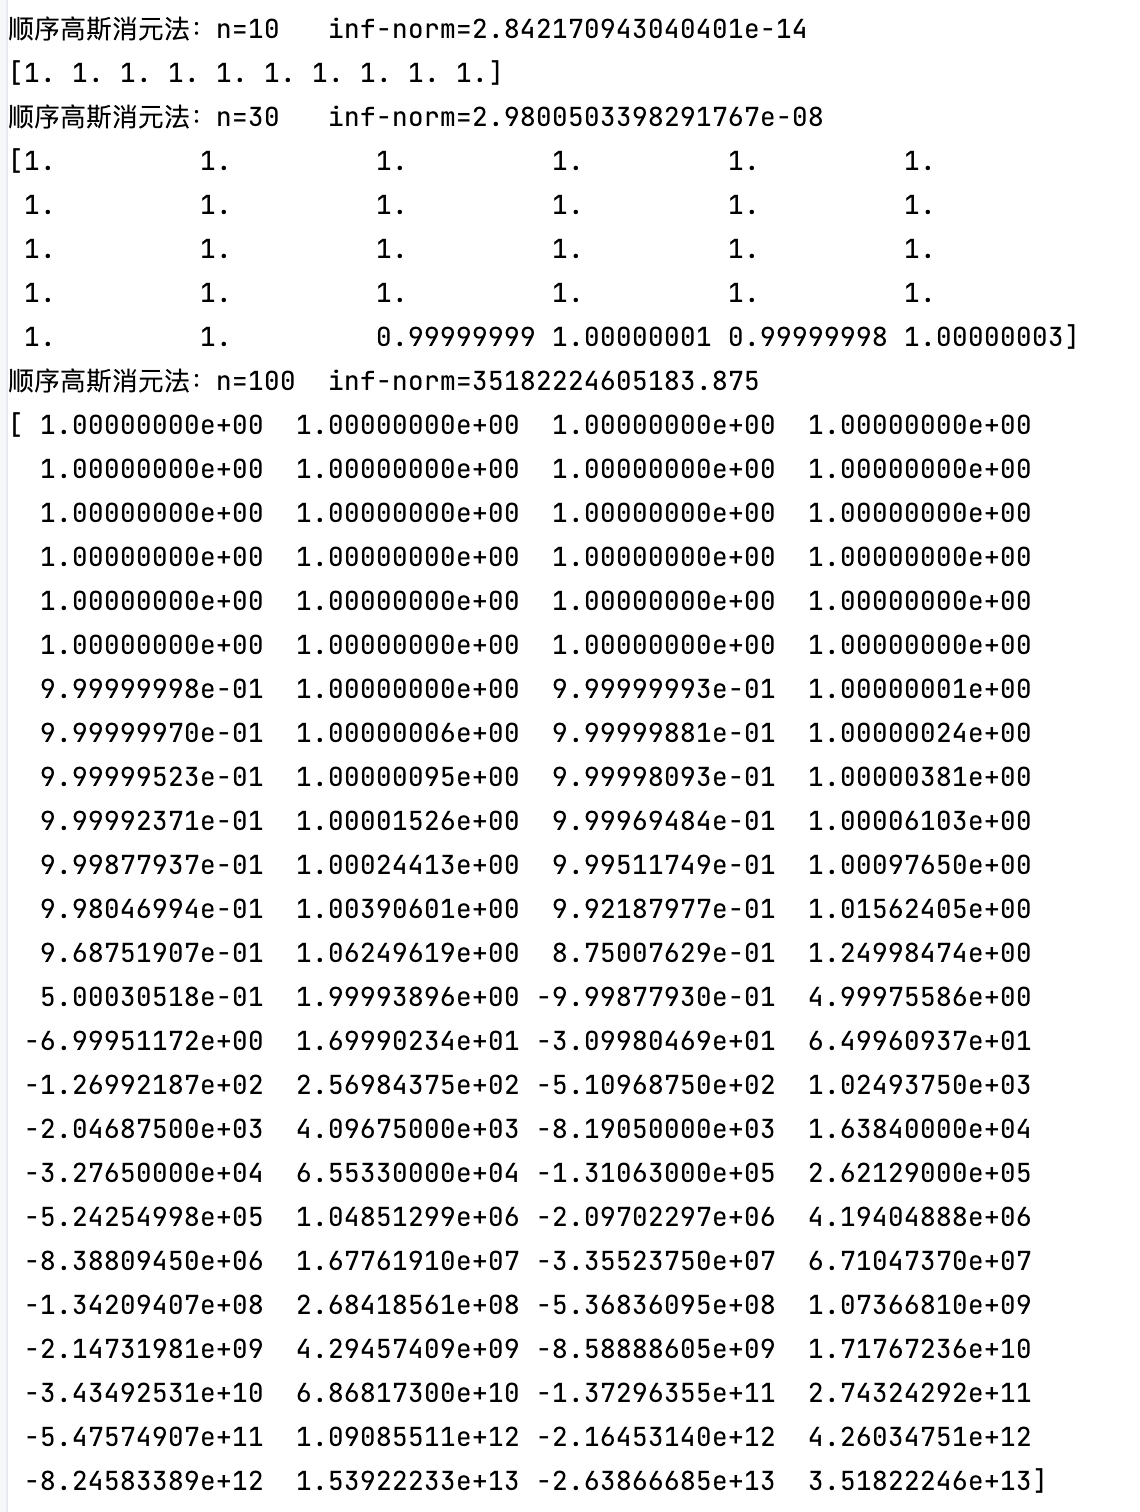
\includegraphics[width=\textwidth]{pic/SeqGuass.png}
\end{minipage}
\begin{minipage}{0.45\textwidth}
    \begin{table}[H]
        \centering
        \caption{顺序 Guass 消元法结果与精确值的比较}
        \begin{tabular}{cc}
            \toprule
            阶数 $n$ & $\infty$-范数 $\lVert \bm{x}-\bm{x}^* \rVert_\infty$ \\
            \midrule
            10  & $2.84\times 10^{-14}$ \\
            30  & $2.98\times 10^{-8}$  \\
            100 & $3.52\times 10^{13}$  \\
            \bottomrule
        \end{tabular}
    \end{table}
    \vspace*{-0.75cm}
    \begin{figure}[H]
        \centering
        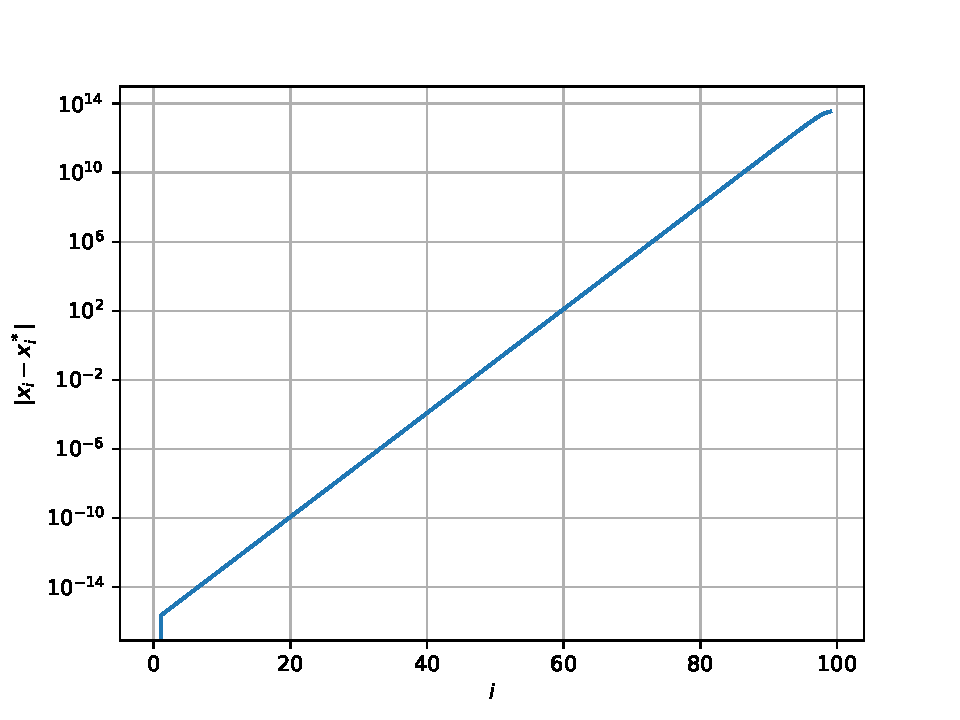
\includegraphics[width=\textwidth]{pic/SeqGuassSolver.pdf}
        \caption{顺序 Guass 消元法 $n=100$ 时结果每个坐标与精确值的差值绝对值}
    \end{figure}
\end{minipage}

\section{列主元 Guass 消元法}

蓝色部分为列主元 Guass 消元法相较于顺序 Guass 消元法增加的代码部分。

\inputminted[firstline=50,lastline=91,highlightlines=60-75]{python3}{main.py}

\begin{minipage}{0.5\textwidth}
    \begin{figure}[H]
        \centering
        \inputminted[firstline=35,lastline=57,fontsize=\tiny]{text}{stdout.txt}
        \caption{列主元 Guass 消元法结果}
    \end{figure}
    % 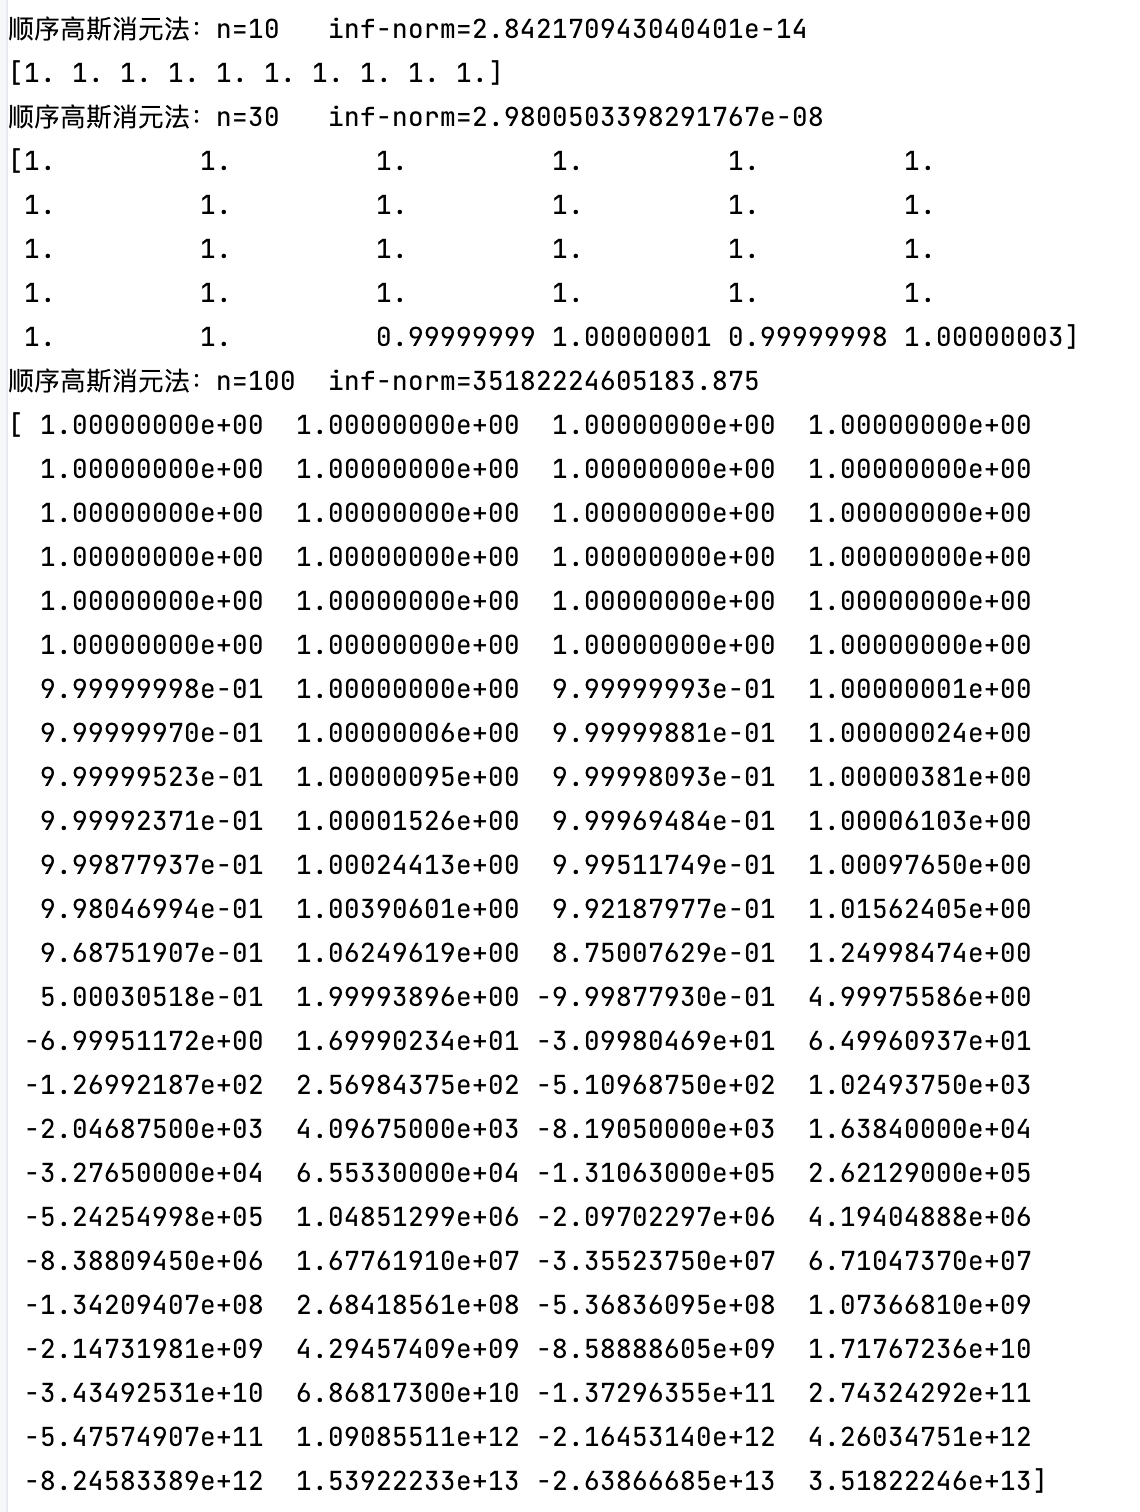
\includegraphics[width=\textwidth]{pic/SeqGuass.png}
\end{minipage}
\begin{minipage}{0.45\textwidth}
    \begin{table}[H]
        \centering
        \caption{列主元 Guass 消元法结果与精确值的比较}
        \begin{tabular}{cc}
            \toprule
            阶数 $n$ & $\infty$-范数 $\lVert \bm{x}-\bm{x}^* \rVert_\infty$ \\
            \midrule
            10  & $0.000$      \\
            30  & $0.000$      \\
            100 & $0.183$\\
            \bottomrule
        \end{tabular}
    \end{table}
    \vspace*{-0.75cm}
    \begin{figure}[H]
        \centering
        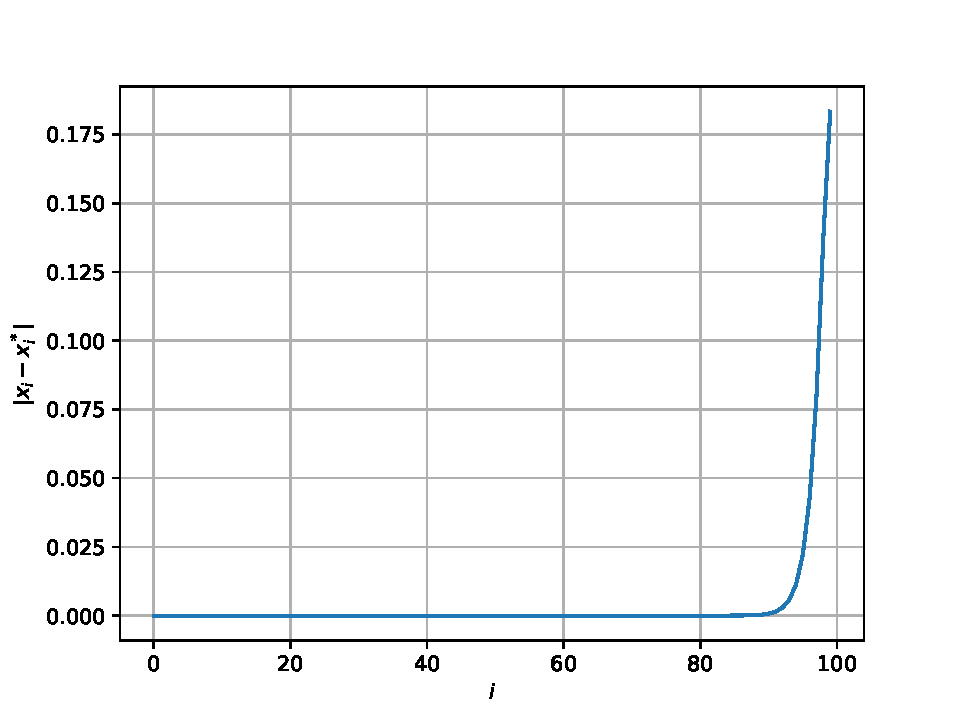
\includegraphics[width=\textwidth]{pic/PivotGuassSolver.pdf}
        \caption{列主元 Guass 消元法 $n=100$ 时结果每个坐标与精确值的差值绝对值}
    \end{figure}
\end{minipage}

\section{追赶法}

追赶法增加了对是否是三对角矩阵以及对角占优矩阵的检查。

\inputminted[firstline=94,lastline=134]{python3}{main.py}
\begin{minipage}{0.5\textwidth}
    \begin{figure}[H]
        \centering
        \inputminted[firstline=58,lastline=94,fontsize=\tiny]{text}{stdout.txt}
        \caption{追赶法结果}
    \end{figure}
    % 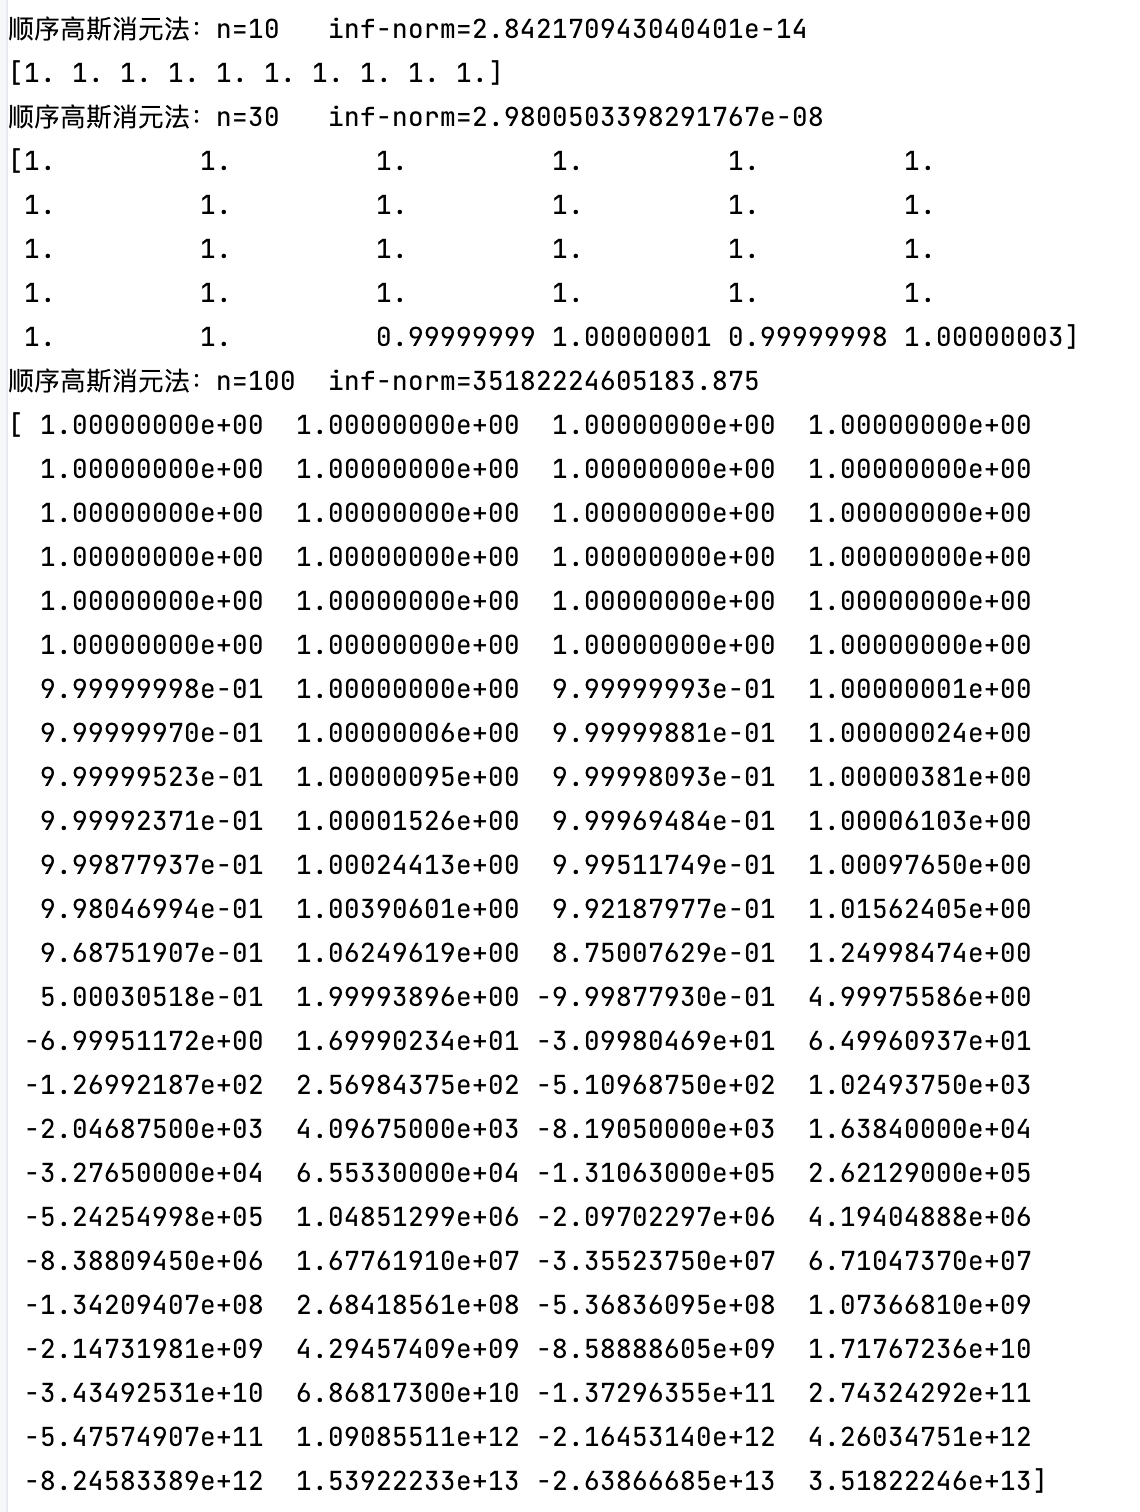
\includegraphics[width=\textwidth]{pic/SeqGuass.png}
\end{minipage}
\begin{minipage}{0.45\textwidth}
    \begin{table}[H]
        \centering
        \caption{追赶法结果与精确值的比较}
        \begin{tabular}{cc}
            \toprule
            阶数 $n$ & $\infty$-范数 $\lVert \bm{x}-\bm{x}^* \rVert_\infty$ \\
            \midrule
            10  & $2.84\times 10^{-14}$ \\
            30  & $2.98\times 10^{-8}$ \\
            100 & $3.52\times 10^{13}$ \\
            \bottomrule
        \end{tabular}
    \end{table}
    \vspace*{-0.75cm}
    \begin{figure}[H]
        \centering
        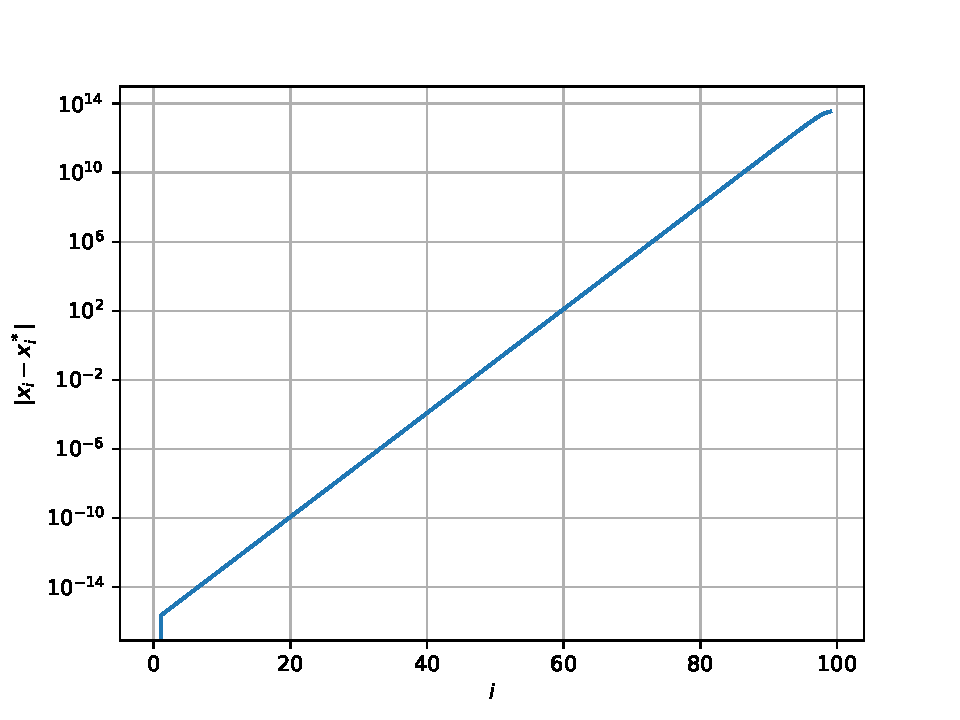
\includegraphics[width=\textwidth]{pic/ThomasSolver.pdf}
        \caption{追赶法 $n=100$ 时结果每个坐标与精确值的差值绝对值}
    \end{figure}
\end{minipage}

\clearpage

\section{Jacobi 迭代法}
\label{sec:jacobi}

\inputminted[firstline=158,lastline=183]{python3}{main.py}
\vspace*{-0.6cm}
\begin{minipage}{0.5\textwidth}
    \begin{figure}[H]
        \centering
        \inputminted[firstline=95,lastline=132,fontsize=\tiny]{text}{stdout.txt}
        \caption{Jacobi 迭代法结果}
    \end{figure}
    % 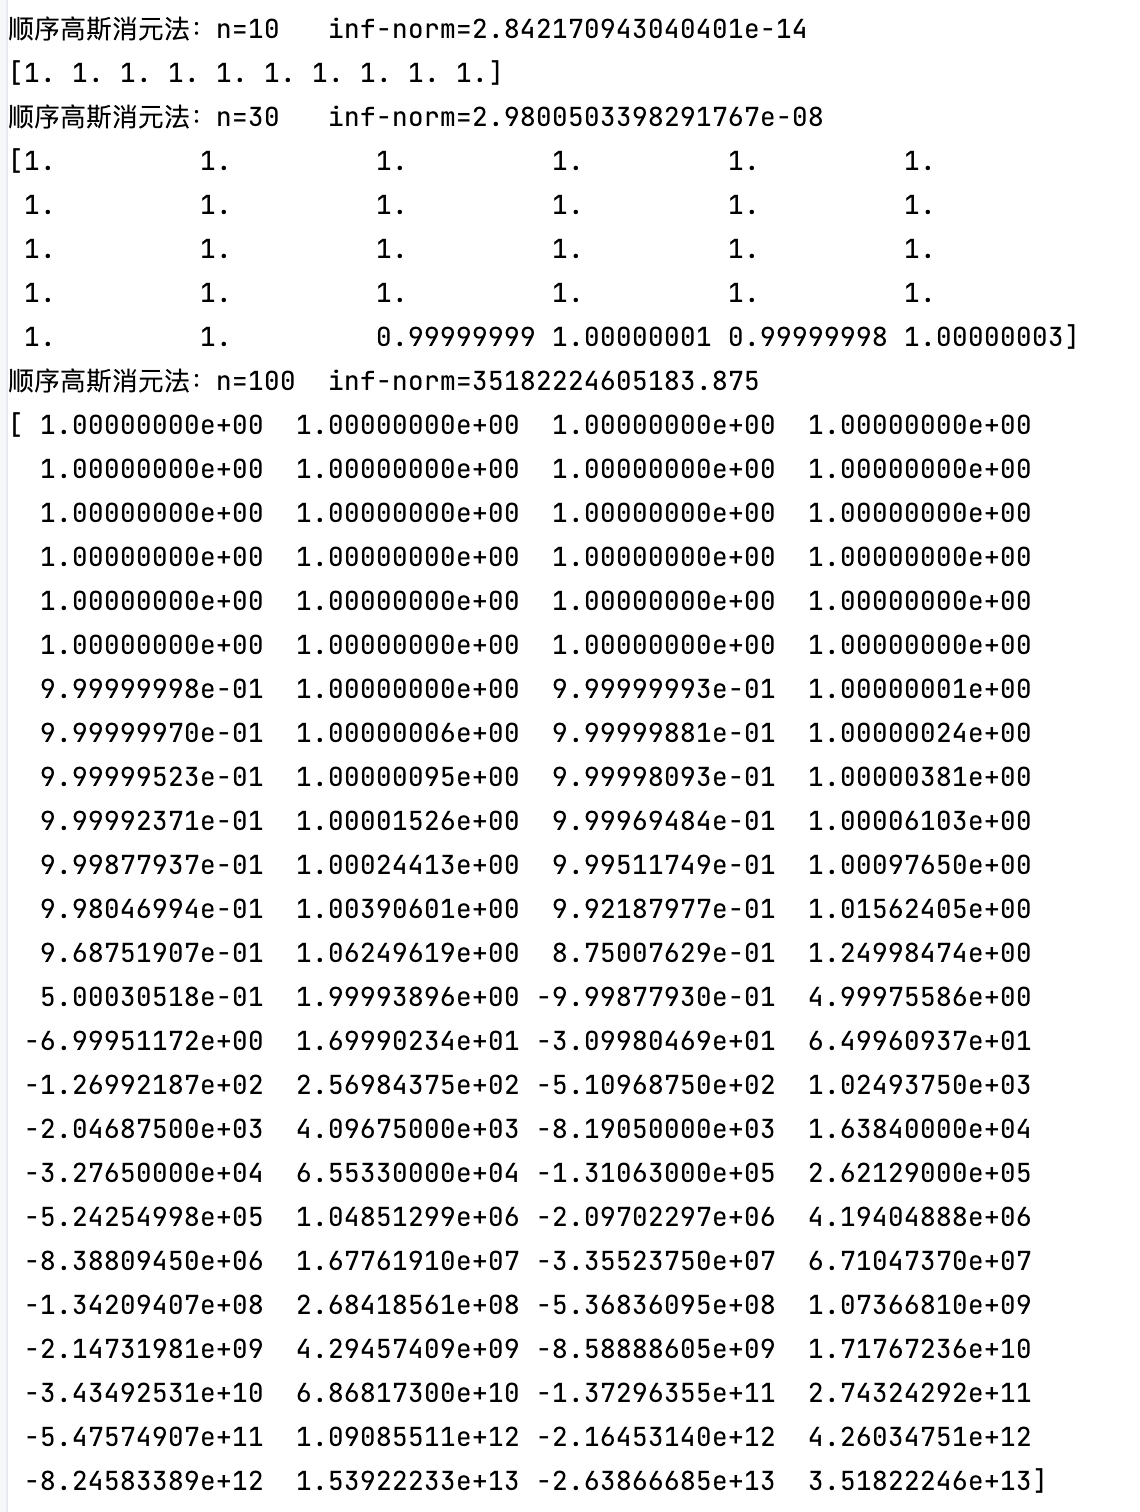
\includegraphics[width=\textwidth]{pic/SeqGuass.png}
\end{minipage}
\begin{minipage}{0.45\textwidth}
    \begin{table}[H]
        \centering
        \caption{Jacobi 迭代法结果与精确值的比较}
        \begin{tabular}{ccc}
            \toprule
            阶数 $n$ & 迭代次数 $T$ & $\infty$-范数 $\lVert \bm{x}-\bm{x}^* \rVert_\infty$ \\
            \midrule
            10 & 159   & $5.59\times 10^{-5}$ \\
            30 & 526   & $3.97\times 10^{-5}$ \\
            100 & 1000 & $1.64\times 10^{14}$\\
            \bottomrule
        \end{tabular}
    \end{table}
    \vspace*{-0.75cm}
    \begin{figure}[H]
        \centering
        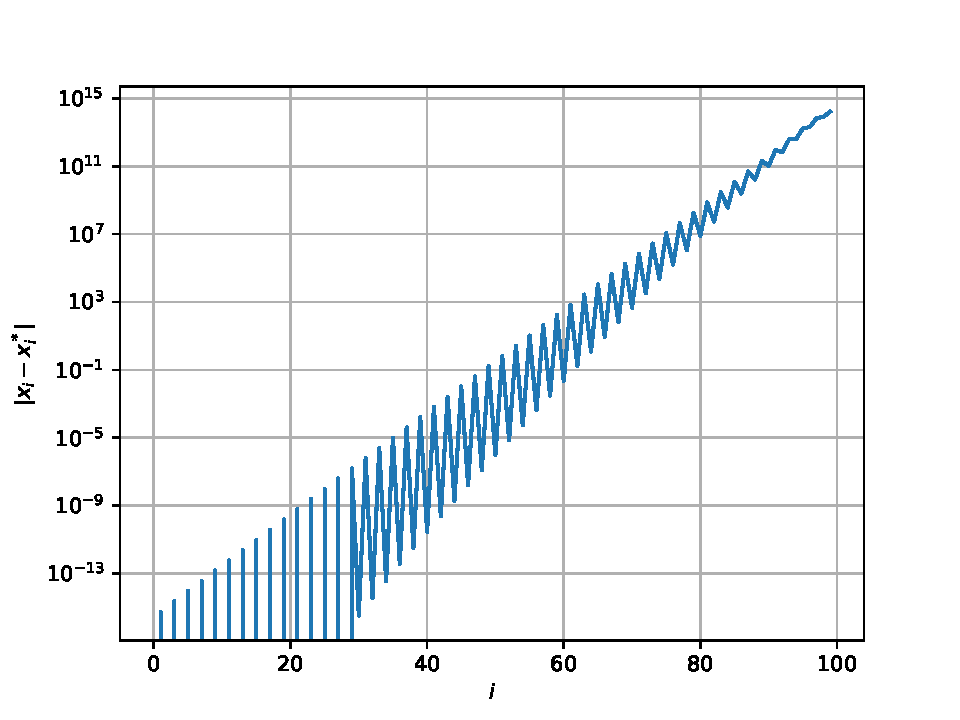
\includegraphics[width=\textwidth]{pic/JacobiSolver.pdf}
        \caption{Jacobi 迭代法 $n=100$ 时结果每个坐标与精确值的差值绝对值}
    \end{figure}
\end{minipage}

\section{Guass--Seidel 迭代法}
\label{sec:gs}

\inputminted[firstline=186,lastline=211,highlightlines=201-204]{python3}{main.py}
\vspace*{-0.6cm}
\begin{minipage}{0.5\textwidth}
    \begin{figure}[H]
        \centering
        \inputminted[firstline=133,lastline=170,fontsize=\tiny]{text}{stdout.txt}
        \caption{Guass--Seidel 迭代法结果}
    \end{figure}
    % 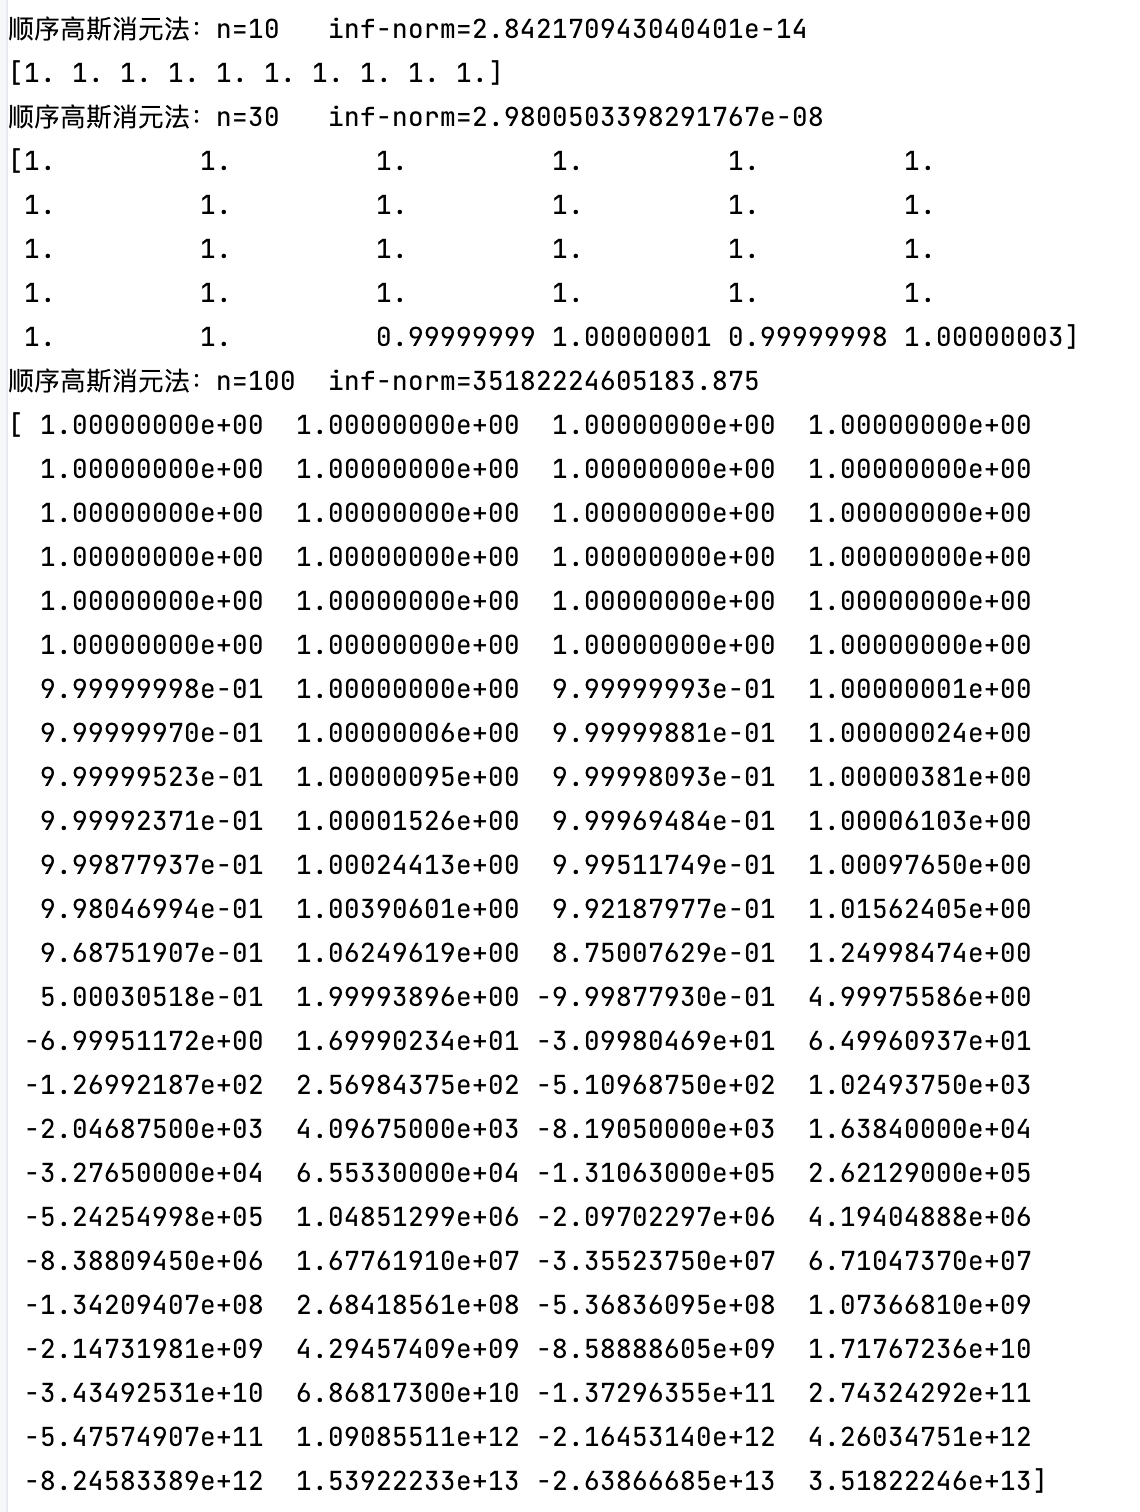
\includegraphics[width=\textwidth]{pic/SeqGuass.png}
\end{minipage}
\begin{minipage}{0.45\textwidth}
    \begin{table}[H]
        \centering
        \caption{Guass--Seidel 迭代法结果与精确值比较}
        \begin{tabular}{ccc}
            \toprule
            阶数 $n$ & 迭代次数 $T$ & $\infty$-范数 $\lVert \bm{x}-\bm{x}^* \rVert_\infty$ \\
            \midrule
            10 & 52   & $0.000431$          \\
            30 & 208  & $0.000690$          \\
            100 & 722 & $9.38\times 10^{13}$\\
            \bottomrule
        \end{tabular}
    \end{table}
    \vspace*{-0.75cm}
    \begin{figure}[H]
        \centering
        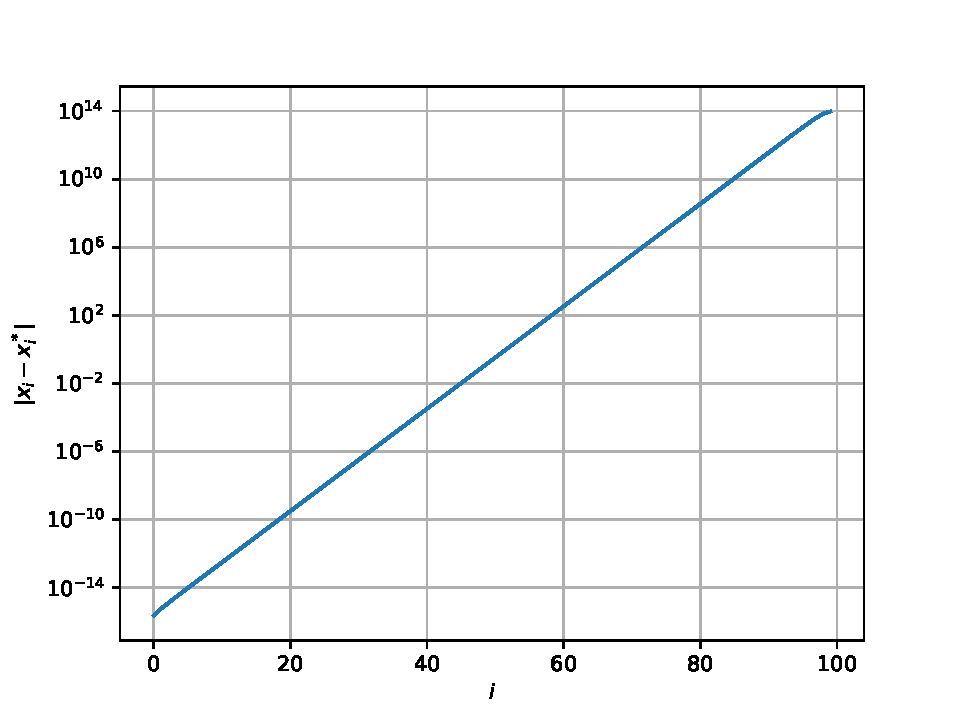
\includegraphics[width=\textwidth]{pic/GuassSeidelSolver.pdf}
        \caption{Guass--Seidel 迭代法 $n=100$ 时结果每个坐标与精确值的差值绝对值}
    \end{figure}
\end{minipage}

蓝色部分为 Guass--Seidel 迭代法相较于 Jacobi 迭代法修改的部分。

\begin{figure}[h]
    \centering
    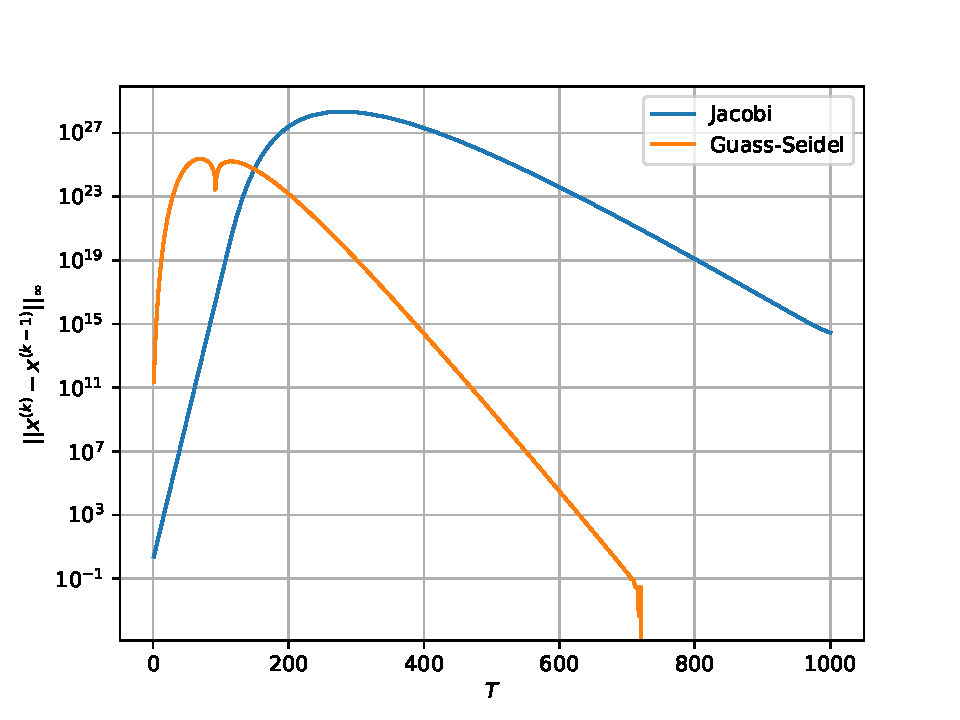
\includegraphics[height=8cm]{pic/iter.pdf}
    \caption{$n=100$,Jacobi 迭代法和 Guass--Seidel 迭代法 $\left\lVert x^{(k)}-x^{(k-1)}\right\rVert_\infty$ 与迭代次数 $T$ 的关系}
    \label{fig:iter}
\end{figure}

\section{结果比较与总结}

首先,分析问题本身的情况。讨论在 $n=10,30,100$ 时矩阵 $\bm{A}$ 的条件数,有表 \ref{tab:cond} 的结果。

\begin{table}[H]
    \centering
    \caption{矩阵条件数}
    \label{tab:cond}
    \begin{tabular}{cc}
        \toprule
        $n$ & $\text{cond}(\bm{A})$ \\
        \midrule
        10 & $1727.556025$ \\
        30 & $1.83702\times 10^9$ \\
        100 & $2.95670\times 10^{16}$ \\
        \bottomrule
    \end{tabular}    
\end{table}

可以看到这个问题本身就是病态的,在 $n=30,100$ 时已经非常病态,容易产生累积误差,也就越难得到方程组准确的解。

\begin{table}[H]
    \centering
    \caption{不同方法结果与准确值的 $\infty$-范数 $\lVert \bm{x}-\bm{x}^* \rVert_\infty$ 比较表}
    \label{tab:res}
    \begin{tabular}{cccccc}
        \toprule
        $n$ & 顺序 Guass 迭代法 & 列主元 Guass 迭代法 & 追赶法 & Jacobi 迭代法 & Guass--Seidel 迭代法 \\
        \midrule
        10  & $2.84\times 10^{-14}$ & $0.000$       & $2.84\times 10^{-14}$ & $5.59\times 10^{-5}$ & $0.000431$           \\
        30  & $2.98\times 10^{-8}$  & $0.000$       & $2.98\times 10^{-8}$  & $3.97\times 10^{-5}$ & $0.000690$           \\
        100 & $3.52\times 10^{13}$  & $0.183$ & $3.52\times 10^{13}$  & $1.64\times 10^{14}$ & $9.38\times 10^{13}$ \\
        \bottomrule
    \end{tabular}
\end{table}

\begin{figure}[h]
\centering
\begin{tikzpicture}
    \begin{semilogyaxis}[grid={both},
    legend pos={outer north east},
    ylabel={$\lVert \bm{x}-\bm{x}^*\rVert_\infty$},
    symbolic x coords={n=10,n=30,n=100}, xtick=data, ymin=1e-15,
    ]
     \pgfplotstableread{diff.dat}{\diff};
     \addplot+ [thick] table[x=n,y=SeqGuass,] {\diff};
     \addplot+ [] table[x=n,y=PivotGuass,] {\diff};
     \addplot+ [] table[x=n,y=Thomas,] {\diff};
     \addplot+ [] table[x=n,y=Jacobi,] {\diff};
     \addplot+ [] table[x=n,y=GuassSeidel,] {\diff};
     \legend{SeqGuass,PivotGuass,Thomas,Jacobi,GuassSeidel,}
    \end{semilogyaxis}
\end{tikzpicture}
\caption{不同方法结果与准确值的 $\infty$-范数 $\lVert \bm{x}-\bm{x}^* \rVert_\infty$ 比较图}
\label{fig:res}
\end{figure}

表 \ref{tab:res} 和图 \ref{fig:res} 展示了不同方法结果与准确值的 $\infty$-范数 $\lVert \bm{x}-\bm{x}^* \rVert_\infty$ 的比较,在 $n=10,n=30$ 时,这些方法结果与准确值的误差都是可以接受的。

对于直接法(顺序 Guass 消元法、列主元 Guass 消元法、追赶法),列主元 Guass 消元法是最优的,尽可能避免了大数除以小数的现象;顺序 Guass 消元法和追赶法结果与准确解的误差一致,但是对于这种特殊的三对角矩阵,追赶法的复杂度为 $O(n)$,比顺序 Guass 消元法、列主元 Guass 消元法的 $O(n^3)$ 下降了不少。

对于迭代法(Jacobi 迭代法、Guass--Seidel 迭代法),图 \ref{fig:iter} 显示了两种方法迭代过程,可见 Guass--Seidel 迭代法比 Jacobi 迭代法收敛更快,Jacobi 迭代法在 $n=100$ 的 1000 轮迭代后仍未收敛。迭代法的时间复杂度为 $O(Tn)$,$T$ 为迭代次数。

从每种方法 $n=100$ 时每个坐标与精确值的差值与绝对值图来看,下标越大,累计的误差越大,呈指数增长。最开始的一些值误差仍在控制范围之内。这就意味着对于这种大型矩阵而言,应当把重要的、精度要求高的变量放在前面(比如主成分分析中的主要成分),以达到更理想的效果。

总之,对于本题,列主元 Guass 消元法的结果是最优的。
\begin{itemize}
    \item 对于大规模矩阵,尽可能地把重要的变量放在前面,
    \begin{itemize}
        \item 对于三对角矩阵这种特殊情况,追赶法可能是运行速度最快的,如果是对角占优的,误差也会被控制;
        \item 当不是三对角矩阵时,为了求解大规模矩阵可以考虑迭代法更快求解;
        \item 合理时间范围内更精确的精度应该超过了这几种方法的范畴,需要进一步地根据实际问题优化;
    \end{itemize}
    \item 对于小规模矩阵,由于顺序 Guass 消元法误差较大且要求对角线元素不为 0、追赶法误差与顺序 Guass 消元法一致,所以一般使用列主元 Guass 消元法精确求解。
\end{itemize}

\end{document}


